\documentclass{article}

% if you need to pass options to natbib, use, e.g.:
%     \PassOptionsToPackage{numbers, compress}{natbib}
% before loading neurips_2019

% ready for submission
% \usepackage{neurips_2019}

% to compile a preprint version, e.g., for submission to arXiv, add add the
% [preprint] option:
\usepackage[preprint]{neurips_2019}

% to compile a camera-ready version, add the [final] option, e.g.:


% to avoid loading the natbib package, add option nonatbib:
%     \usepackage[nonatbib]{neurips_2019}

\usepackage[utf8]{inputenc} % allow utf-8 input
\usepackage[T1]{fontenc}    % use 8-bit T1 fonts
\usepackage{hyperref}       % hyperlinks
\usepackage{url}            % simple URL typesetting
\usepackage{booktabs}       % professional-quality tables
\usepackage{amsfonts}       % blackboard math symbols
\usepackage{nicefrac}       % compact symbols for 1/2, etc.
\usepackage{microtype}      % microtypography
\usepackage[utf8]{inputenc}
\usepackage{amsmath}
\usepackage{amsfonts}
\usepackage{amssymb}
\usepackage{mathtools}
\usepackage{listings}
% \usepackage{graphicx}
\usepackage{caption}
\captionsetup{width=.9\textwidth}
\usepackage{subcaption}
\usepackage{float}
\setlength{\parskip}{\baselineskip}
\setlength{\parindent}{0cm}
\usepackage{xcolor}
\usepackage{enumitem}
\usepackage[backend=bibtex,style=verbose-trad2]{biblatex}
\title{Apply Prior Knowledge in Motif Finding with MEME}
\usepackage{subfigure}
\usepackage{algorithm}
\usepackage{algorithmic}
\usepackage{algpseudocode}% http://ctan.org/pkg/algorithmicx
% The \author macro works with any number of authors. There are two commands
% used to separate the names and addresses of multiple authors: \And and \AND.
%
% Using \And between authors leaves it to LaTeX to determine where to break the
% lines. Using \AND forces a line break at that point. So, if LaTeX puts 3 of 4
% authors names on the first line, and the last on the second line, try using
% \AND instead of \And before the third author name.

\author{%
  Xingyu Chen\ \\
  Department of Computer Science\\
  Cornell University\\
  Ithaca, NY 14850 \\
  \texttt{\{xc374}@cornell.edu\}}



\begin{document}

\maketitle

\section{Introduction}

Motif finding is a primary step in studying gene function and plays a vital role in learning the mechanisms for regulation of gene expressions. For instance, the shared biological function could be explained by motif subsequences as evidence and could be utilized into finding common protein binding sites or splice junctions in DNA sequence or the active site of relevant enzymes in RNA sequence (Bailey and Elkan, 1994).

Although lots of algorithms has been extended, this task still remains challenging. There are mainly two types of motif finding algorithms: the enumeration approach and probabilistic approach. The enumeration approach search motif based on enumeration of words and computing similarity (Hashim et al. 2019). The probabilistic approach constructs the Position Weight Matrix (PWM) that specifies base distribution to distinguish background and motifs. The probabilistic approaches include stochastic method and deterministic method. One popular stochastic method is the Markov chain Monte Carlo (MCMC) that optimizes PWM using Gibbs sampling by iteratively generating new motif start positions (Bi 2009). The deterministic method instead uses Expectation Maximisation to find optimum PWM. This project describes a deterministic method called MEME to discover several different motifs of differing and unknown width in a single DNA or protein dataset. 


\section{Overview of MEME}
In the first version of MEME algorithm, the exact motif length are specified as one of its input parameters (Bailey and Elkan, 1994). At each pass of the algorithm, it will compute a motif of fixed length and it is not able to find multiple motifs with different lengths with a single run of the algorithm. Also, another limitation of MEME is that it requires multiple runs of the algorithm with random start points to avoid hitting local optima caused by running the EM algorithm.  In this project, a modified MEME algorithm proposed in (Bailey and Elkan, 1995b), which is the third version of MEME, will be implemented to overcome those limitations in the early versions of MEME. Specifically, the innovations will include 

(1) Use of Dirichlet mixture priors to initialize PWM.

(2) A global search algorithm 'TEST' based on approximated EM heuristics for choosing optimum starts points for MEME. 

(3) A Likelihood Ratio Test (LRT) based method to auto determine best width of the motifs. 

(4) A new type of sequence model called ZOOPS to allow each sequence in the training set to have zero or one occurrences of each motif. 

In general, the MEME algorithms find a different motif with optimum width at each pass and by specifying the number of pass for running MEME, multiple motifs could be found based on EM algorithm. It determines good start points and avoids being stuck at local optima running EM without repeatedly re-running from different random starting points. To weight importance of motifs between different width, the likelihood metric cannot be used directly since the number of free model parameters are different due to the difference in width. The Likelihood Ratio Test (LRT) heuristics considers both the likelihood and the number of free parameters into scoring. Above all, same as its early versions, this MEME algorithm eliminates the best founded motif 'probabilistic-ally' at a time and avoids rediscovery of the same motif in the process of find succeeding optimum motifs.  


\section{Model}
There are three types of models supported by MEME specifically the OOPS, the ZOOPS and the TCM models.

\textbf{OOPS}: One Occurrence Per Sequence model. This model assumes there is exactly one occurrence per sequence of motif in the dataset.

\textbf{ZOOPS}: Zero Or One Per Sequence model. This model assumes zero or one motif occurrences per sequence.

\textbf{TCM}: Two Component Mixture model. This model assume that there are zero or more non-overlapping occurrences of the same motif in the sequence. For example, given a sequence of 'ATGCTTgggccATGCTT', the model is able to detect multiple occurrences of the motif 'ATGCTT' at the same sequence. 

In the project, only the OOPS and ZOOPS model are implemented and discussed. Both model consist of two components. The motif and background positions in the sequences. The parameters associated with these model are 

\begin{align*}
\theta &= \begin{bmatrix} \theta_0 & \theta_1\end{bmatrix}= \begin{bmatrix} p_0 & p_1 & p_2 & ... & p_W\end{bmatrix}\\
&=
\begin{bmatrix}
P_{A,0} & P_{A,1} & P_{A,2}&...& P_{A,W} \\
P_{G,0}& P_{G,1}& P_{G,2}&...& P_{G,W}\\
P_{C,0}& P_{C,1}& P_{C,2}&...& P_{C,W} \\
P_{T,0} & P_{T,}& P_{T,2}&...& P_{T,W}
\end{bmatrix}
\end{align*}

The alphabet for the sequences in this project is ${A,G,C,T}$. Hence, $P_{x,j}$ is the probability of letter x occurring at a background if $j=0$ or at at motif position j if $1<=j<=W$. 

Additionally, the ZOOPS model incorporate a new parameter $\gamma$ - the prior the prior probability of a sequence model containing a motif occurrence. Thus, assume a sequence of length $L$ and motif length of $W$, the number of possible motif start position is $m$, where $m=L-W+1$, thereby the prior probability of a sequence model contain a motif starting at either one of the $m$ possible position could be expressed as  $\lambda$, where $\lambda=\frac{\gamma}{m}$. In OOPS model, the $\gamma$ is simply set as constant 1 and $\lamba$ is set as$\frac{1}{m}$.


\section{Training}
The dataset contains n sequences of different length as $X ={X_1,X_2,...X_n}$. The model includes an indicator variable called the 'missing information' denoted by $Z$, where $Z_{ij}$=0 meaning a motif starts at position $j$ of $X_i$. The ZOOPS model introduces another indicator variable $Q$, where $Q_i=\sum_{i}^{m}Z_{ij}$. $Q_i=0$ meaning sequence $X_i$ does not contain any motif. 

To compute the optimum starting point of motif, the model runs an EM algorithm. On a high level, the E step is to variable $Z$ and M step is to update the each column of PWM matrix $p_k$ $(1<=k<=W$  and $p_0$.  The detailed update rule is shown below.
\subsection{Conditional Probability}
Here lists the conditional probabilities used in the EM steps.

\begin{equation}
\begin{split}
\log{Pr(X,Z|\theta,\lambda)}=\sum_{k=0}^{W-1}\textbf{I}(i,j+k)^T\log{p_k}+\sum_{k\in\Delta_{i,j}}\textbf{I}(i,k)^T\log{p_0}\\
\Delta_{i,j}  = {1,2,..,j-1,j+w,...L}
\end{split}
\end{equation}

where ${I}(i,j)$ is a indicator vector to indicate the corresponding letter among ${A,T,C,G}$ at position $j$ of sequence $X_i$.  $\Delta_{i,j}$  is the set of non-motifs positions if the motif starts at at position $X_i_j$.

The conditional probability of a length-W sub sequence being the background component or the motif component could be defined as
\begin{align}
\log{Pr(X_{ij}|\theta_c)}=\sum_{k=0}^{W-1}\textbf{I}(i,j+k)^T\log{p_{k^{'}}}\end{align}
where $k^{'}=0$ of $c=0$ otherwise $k^{'}=k+1$ with  $c=1$ . 

The conditional probability of a sequence taht does not contain motif under the ZOOPS model could be defined as
\begin{align}
\log{Pr(X_{i}|Q_i=0,\theta)}=\sum_{k=0}^{L-1}\textbf{I}(i,j+k)^T\log{p_{0}}\end{align}
\subsection{The E-step}
The E-step is to calcualte the expected value of $Z$. For the OOPs model:
\begin{align}
Z^{(t)}_{i,j}=\frac{Pr(X|Z_{i,j}=1,\theta^{(t)}}{\sum_{j=1}^{m}Pr(X|Z_{i,j}=1,\theta^{(t)}}
\end{align}

For the ZOOPS model,

\begin{align}
Z^{(t)}_{i,j}&=\frac{Pr(X|Z_{i,j}=1,\theta^{(t)}}{\sum_{j=1}^{m}Pr(X|Z_{i,j}=1,\theta^{(t)}},\\
f_0&=Pr(X_i|Q_{i}=0,\theta^{(t)}(1-\gamma^{(t)}) \\
f_1&=Pr(X_i|Z_{i,j}=1,\theta^{(t)}\lambda^{(t)}), 1\leq j\leq m
\end{align}

\subsection{The M-step}
The M-step of EM will re-estimate the PWM matrix and background probability following the formula below

\begin{align}\label{eqn}
p_k^{(t+1)}&=\frac{c_k+d_k}{c_k+d_k}, 0\leq k \leq W, \text{where} \\
 c_{k} &=    \begin{cases}
      t-\sum_{j=1}^{W}c_j & \text{if $k$ = 0}\\ 
      \sum_{i=1}^{n}\sum_{j=1}^{m}Z^{(t)}_{i,j}\textbf{I}(i,j+k-1)^T & \text{otherwise}
    \end{cases} 
\end{align}

Here, $d_k$ could be seen as pseudo-counts to avoid zero probability in the updating process. It could also be viewed as a prior value that incorporates knowledge about motif columns, which will be discussed later. For ZOOPS model, the parameter $\gamma$ and $\lambda$ should be updated in the M step as well using the formula
\begin{align}
\lambda^{(t+1)}=\frac{\gamma^{(t+1)}}{m}=\frac{1}{nm}\sum_{i=1}^{n}\sum_{j=1}^{m}Z^{(t)}_{i,j}
\end{align}

\subsection{Scoring}
\textbf{EM terminating criterion}

In order to score the generated motif set for the entire sequence, the joint likelihood function should be computed as it will be used in computing LRT statistics. The joint likelihood is typically used as the terminated criteria to the EM process. 

One solution is to monitor the level-off of the joint likelihood value. Additionally, we could also use the change of PWM matrix $P_k$ (1<=k<=W) as stop criterion, which is the practical criterion being implemented in MEME suite [7]. The absolute value of difference of PWM with the last iteration should be zero upon convergence.  The formula to calculate joint likelihood for OOPS model is given by:
\begin{align}
\log{Pr(X,Z|\theta)}=\sum_{i=1}^{n}\sum_{j=1}^{m}\log{Pr(X_i|Z_{i,j}=1,\theta)}+n\log{\frac{1}{m}}
\end{align}
For a ZOOPS model, the formula is
\begin{equation}
\begin{split}
\log{Pr(X,Z|\theta)}&=\sum_{i=1}^{n}\sum_{j=1}^{m}\log{Pr(X_i|Z_{i,j}=1,\theta)}\\&+\sum_{i=1}^{n}(1-Q_i)\log{Pr(X_i|Q_i=0,\theta)}\\
&+\sum_{i=1}^{n}(1-Q_i)\log{(1-\gamma_i)}+\sum_{i=1}^{n}Q_i\log{\lambda_i}
\end{split}
\end{equation}
\textbf{Determining the Best Width}

Given the input sequences, converged $\theta_0$, $\theta_1$ and $\gamma$, the paper uses a Likelihood Ratio Test, they compute a chi-square statistics using a null model and an alternative model, based on the formula below:
\begin{equation}
\begin{split}
\chi^2&=-2\log{\frac{Pr(X|\phi_0)}{Pr(X|\pho)}}, \text{where}\\ 
\log{Pr(X|\phi_0)} &=nL\sum_{s\in{L}}{\mu_x\log\mu_x}  \\
\log{Pr(X|\phi)}&= \log{Pr(X,Z|\theta)}
\end{split}
\end{equation}
Here, $\mu$ is the vector of average letter frequency of the dataset. 

The significance level $LRT(\phi)$ could be defined and approximated using standard normal distribution $Q$:
\begin{equation}
\begin{split}
LRT(\Phi)=Q(\lambda^2|\upsilon)\approx Q(\frac{(\chi^{2}/\upsilon)^{\frac{1}{3}}-(1-\frac{2}{9\upsilon})}{\sqrt{2/(9\upsilon)}})
\end{split}
\end{equation}
where $\upsilon$ is the different in free parameters. There are $(4-1)$ free parameter per column of $\theta$ so  $\upsilon= 3W$.
The final criterion function is to \textbf{minimize} a significance score noted by $G(\phi)$, which imposes a penalty on $\upsilon$, defined by
\begin{equation}
\begin{split}
\log(G(\Phi))=\frac{1}{v}\log(LRT(\Phi))
\end{split}
\end{equation}
This is ideal, since if only using joint-likelihood as criterion, then a shorter motif width is always be favoured due to the difference of free parameters. By minimizing this new criterion $G$, a shorter motif W, will impose a larger penalty since there more free parameters defined by $\upsilon$. 


\subsection{Motif Eraser}
The section above summaries the steps used in a single pass of MEME, which is for detecting a single type of motif from the sequences. The most important algorithm is what I called the 'motif eraser', which will be applied after each motif for a particular width is found, this is called a \textbf{pass} of MEME. It will 'erase' the motif 'probabilistic-ally' as if it is not in the sequence. In theory, the approach used by MEME to find multiple motifs at different passes is the greedy search algorithm. Initially, MEME assumes $Pr(Z_i_j=1)=\lambda$ for all $Z_i_j$. In the subsequent passes of MEME, a new prior on each $Z_i_j$ will be computed in the E step and takes into account a new motif of width $W$ starting at each position might overlap the occurrences of the motifs found previously.
Mathematically, to update the $Z$ variable to include previous founded motif position, a variable $V$ is introduced. 
\begin{align}
V_{ij} &=    \begin{cases}
      1 & \text{if no old motifs in $[X_j,...,X_{j+w-1}]$}\\
      0 & \text{otherwise}
      \end{cases}
\end{align}
for $i=1,...n$ and $j=1,...,m$.

To compute $V$, a binary variable $U$ - an indicator of which positions are not contained in occurrences of previously found motifs

\begin{align}
U_{ij} &=    \begin{cases}
      1 & \text{if $X_{i,j}$ $\notin$ previously founded motifs}\\
      0 & \text{otherwise}
  \end{cases}
\end{align}

for $i=1,...n$ and $j=1,...,m$.

This variable $U$ is updated after each pass of MEME with the formula:
\begin{align}
U_{ij}^{p} =U_{ij}^{p-1}(1- \max_{k={j-W+1,...,j}}{Z_{i,k}^{(t)}})
\end{align}
The maximum of $Z_i_j$ is used because $Z_i_j$ is not independent with each other since current motif cannot overlap themselves. The value of $U_{ij}^{p}$ will be used as the value for $Pr(U_{i,j}=1)$ in the next pass $p+1$. Then we can estimate the $Pr(V_i_j=1)$ as
\begin{align}
Pr(V_i_j=1) =\min_{k={j,...,j+W-1}}{Pr(U_{i,j}=1)}
\end{align}
Note, Initially, $Pr(V_{i,j}=1)=1$ . Thus, we can get the formula for updating the Z in the E-step using the formula:
\begin{align}
\tilde{Z}^{(t)}_{i,j}=Z^{(t)}_{i,j}{Pr(V_{i,j}=1)}
\end{align}
Note that this new $\tilde{Z}$ will be used in place of $Z^{(t)}$ in the M step of EM process in equation (9) and (10) as well as updating $U$ variable in equation (18).

\section{Avoid local minima using Prior Information}
The ideal outcome of MEME is to find the sequence motif that globally maximizes the likelihood. For ZOOPS model, The inner loop of MEME will start EM process from a geometric series of initial $\lambda$. For a ZOOPS model of given width, the MEME finds and runs EM to converge from $\log_2{\sqrt{n}}$ starting point. Assuming there are $K$ different of $W$ and $R$ different $\lambda$ to evaluate, it will start running EM from a optimum start point for a given $\lambda$ (the optimum of a start point is tested using a 'TEST' algorithm). Having different $\lambda$ as starting point considers only a proportion of sequences might contain the motifs. For a give width, it will converge to $R$ different parameter sets including $Z$ and $\theta$. Thus, at each pass it will converge to $R\times K$ different parameters. Among them, based on the criterion $G(\Phi)$ defined in equation (15), only the motifs with best width $W$ and $\lambda$ will be output ed and used to update $U$ for motif eraser in the next pass. 


There are two different $\beta$ (prior) user could tune and set: (1) the initial prior to instantiate the initial PWM matrix which determines the 'size' of the prior and 'fuzziness' of the initialize estimate of the PWM matrix and (2) the prior that incorporates likely motif column knowledge, specifically the $d_k$ term in equation (8). 


\textbf{Initial prior} 

Thus, good stating points are essential for fast convergence and precisely evaluating the importance of a motif width with a specific $\lambda$. The starting point is generated using a Dirichlet prior with a uniform distribution
$\beta$=$[0.2,0.2,0.2,0.2]$, then the initial estimate of sequence to theta prior $p^{(0)}$ could be expressed as 
\begin{align*}
p^{(0)} = [p_{A}^{(0)},p_{C}^{(0)},p_{G}^{(0)},p_{T}^{(0)}]=\begin{bmatrix}
1.2/1.8 & 0.2/1.8 & 0.2/1.8&0.2/1.8 \\
0.2/1.8& 1.2/1.8&0.2/1.8&0.2/1.8\\
0.2/1.8& 0.2/1.8&1.2/1.8&0.2/1.8 \\
0.2/1.8 &0.2/1.8& 0.2/1.8&1.2/1.8
\end{bmatrix}
\end{align*}
There, if a subseqenece $TGTCAT$ of With 6 is chosen as starting points then its initial $theta_1$ is
\begin{align*}
p^{(0)} = [p_{T}^{(0)},p_{G}^{(0)},p_{T}^{(0)},p_{C}^{(0)},p_{A}^{(0)},p_{T}^{(0)}]=\begin{bmatrix}
0.2/1.8 & 0.2/1.8 & 0.2/1.8&0.2/1.8 &1.2/1.8 &0.2/1.8\\
0.2/1.8& 0.2/1.8&0.2/1.8&1.2/1.8 & 0.2/1.8&0.2/1.8\\
0.2/1.8& 1.2/1.8&0.2/1.8&0.2/1.8  &0.2/1.8 &0.2/1.8\\
1.2/1.8 &0.2/1.8& 1.2/1.8&0.2/1.8 &0.2/1.8 &1.2/1.8
\end{bmatrix}
\end{align*}
User can change the value and distribution of $beta$ being used in computing  $p^{(0)}$,

\textbf{Motif knowledge prior}

The prior knowledge could be applied since different letters to the sequence might have different probabilities to occur given the sequence. The motif knowledge prior will be modelled with the equation below using a R-component mixture prior:

\begin{align}
     d_x^k= \sum_{i=1}^{R}Pr(\beta^{(j)}|c_k)\beta_{x}^{(j)}
\end{align}
where $x$ is the letter in the alphabet and $k$ is column of the motif. In this project, only DNA sequences are tested with the MEME, the implemented prior uses a 1-component prior where $R=1$ and for protein based sequence a 30-component prior is used to model the prior. With a 1-component prior, the beta for a column $k$ becomes $[\beta_A^k,\beta_C^k,\beta_G^k,\beta_T^k]$. Often this could be set as the average frequency of letter in the dataset. In this report, different $\beta$ will be evaluated in terms of accuracy of finding motifs.





\textbf{'TEST' algorithm}

The paper also proposes an algorithm to generate optimum starting $\theta_1$ for running MEME. This algorithms will iterate all the possible subsequences for a given motif width and $\lambda$ and estimate  the soundness of $\theta_1$ after one pass of EM using likelihood of the model using the conditional probability  $Pr(X_{i,j}|\theta)$ defined in equation (2). Note that this single iteration of EM is different with the EM in the MEME. It is a approximated EM process and uses $Pr(X_{i,j}|\theta)$ to approximate the expected value of $Z$ and uses the maximum likelihood (looking at the one start position for a sequence) of being motif occurrences to compute letter count to calculate $\theta_1$, rather than 'softly' computing the joint likelihood and considering every possible staring position in the sequence. Thus, this approximated EM process is much faster. Furthermore, I utilized \textbf{dynamic programming} to implement the calculation of $Pr(X_{i,j}|\theta$ in making it even faster and saves a huge amount of computation power. The detailed recursion rule could be found in the technique report from Bailey and Elkan, 1995b. Also, this algorithm is implemented to test several starting $\lambda$ for a given $W$ at once. 
\begin{figure}[H]
\centering
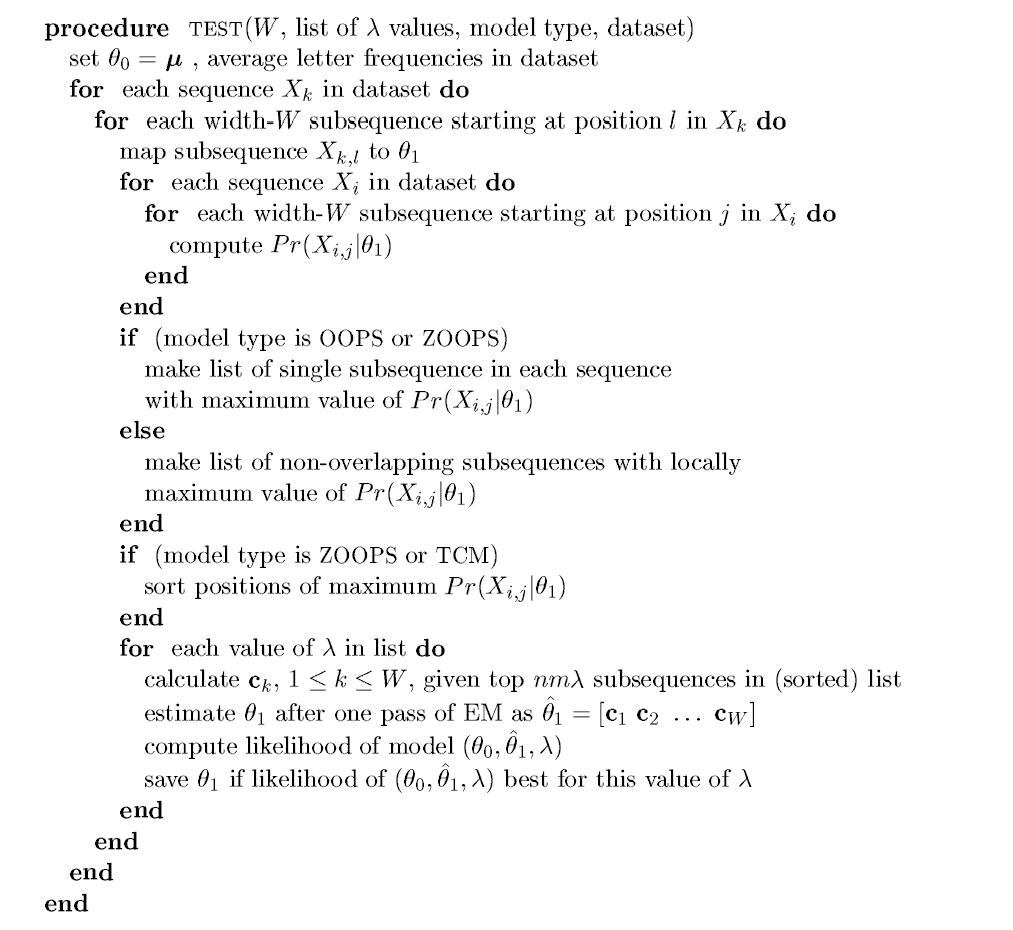
\includegraphics[scale=0.4]{test.jpg}
\captionsetup{width=.8\linewidth}
\caption{TEST Algorithm (Bailey and Elkan, 1995b)}
\label{fig:1}
\end{figure}
\begin{algorithm}
\caption{MEME}
\REQUIRE $\lambda_{min}=1/(m\sqrt{n}), \lambda_{max}=1/m$, input sequence $X$,$pass_{max}$
\For {$W = W_{min}$ \textbf{to} $W = W_{max}$ by $+1$}
    \State {Running TEST(X,a list of $\lambda$, W) and store $\theta$}
\EndFor
\For {$pass = 1$ \textbf{to} $pass_{max}$} 
    \For{$W = W_{min}$ to $W = W_{max}$ by $+1$}
        \For{$\lambda$ = $\lambda_{min}$ to $\lambda$ = $\lambda_{max}$  by $\times\sqrt(2)$}
            \State{Initialize $\theta$  by the stored value from 'TEST' for Width $W$}
            \State{Run EM till convergence from chosen $\phi$ =$(\theta, \lambda, W)$  }
            \State {Compute $G(\phi)$ for given $W$ and $\lambda$}
        \EndFor
    \EndFor
    \State{Find the motif width $W$ that minimizes $G(\phi)$}
    \State{Update the prior probabilities $U_i_j$ to approximate multiple motif model  }
\EndFor
\State \Return {$\theta_1$}
\end{algorithm}
\quad\quad\quad\quad\quad\quad\quad\quad\quad\quad Chart 1. MEME algorithm flowchart
\section{Inference and Evaluation}
\subsection{Inference}
In this project, the inference stage of MEME of motif finding process is entirely based on the missing information $Z$. The missing information during the process is a expected variable so it requires setting a threshold to turn it into a 'hit' only if the normalized Z variable exceeds $0.5$ rather than a simple 'argmax' operation. This will ensure more confidence to the predicted motif sequence. 
The original paper uses a slight different approach which is worthy of mentioning here. Rather than using the intermediate result of Z information at each pass. It uses the PWM matrix $\theta_1$ to evaluate all the sub sequences using a score function and a threshold based on $\lambda$ and finding the start position with the best score among the positions that exceeds the threshold. This is quite interesting and it is more robust than entirely based on the Z variable. I will implement it if I have more time.
\subsection{Metrics}
The evaluation metric uses in the experiment could be divided into two categories, \textbf{motif level metric} and \textbf{sequence level metric}. The sequence level metric are evaluating the robustness of each predicted given the truth motif in the data. The data level metric will evaluate the prediction based on the match of the all the predicted motifs with the truth motifs at each pass of MEME. 

The motif level metrics include:

\begin{enumerate}[label=(\Alph*)]
\item Log Likelihood. Log likelihood of the motif defined by $\log{Pr(X,Z|θ,\lambda)}+\log{(\lambda)}$\\
\item P value of the motif, obtained by running a likelihood test on chi-square distribution with the likelihood for null hypothesis being the motif background probability.\\
\item Character-level precision, this is a self-defined metric based on number of continuous letter overlaps with respect to the true motif. Assuming the predicted sites of the motif is $ATTTGC$ and the true motif is $TTTGCGCGC$, then the number of exact overlapping segment is $TTTGC$. The character-level precision would be the length of overlap divided by the length of prediction which is $5/6$ in this case. Note that for a sequence that have multiple truth motifs, I use the highest score among them.\\

\item Character-level recall. Computed similarly as (C) but focusing on recall statistics. The character-level precision would be the length of overlap divided by the length of truth motif which is $5/9$ for example made in (C).\\

\item Z score: converged expected $Z$ value at the estimated start point, ideally this should be close to 1

\end{enumerate}
The sequence level metrics include:
\begin{enumerate}[label=(\Alph*)]
\item Accuracy. Accuracy score computed based on matched count of motifs across the entire dataset at each pass.
\item ROC statistics. Area under the ROC curve obtained by numerically integrating true positive proportion over false positive proportion (tpp and fpp are obtained as based on matched count of motifs). I followed the same pattern in the paper that each account or each hit is not obtained via exact but a partial match with a shift width allowance.Thus, if the predicted motif start point is a shift version of the truth motif by some allowable amount then it could be account as true positive count.  
\item Avg char precision: averaged motif character-level precision at each pass  
\item Avg char recall: averaged motif character-level recall at each pass  
\end{enumerate}

\section{Result}
The evaluated motif data contain a simulated toy dataset with two truth motif per sequence for testing the algorithm and 3 real datasets on E. coli DNA including crp,lex, crplex as described in (Bailey & Elkan 1995a). The crp sequences contain binding sites for CRP motif and have variable amount of motif occurrence at each sequences. The lex dataset contain motif LexA and two of the input sequences does not contain any motif while the remaining contains a variable amount of motifs at each sequence.The crplex is the union of the crp and lex datasets.

Also, I generated added variable number of random sequences to the crp dataset. For example, the data file 'crp5.fa' appends 5 random sequences and 'crp50.fa' appends 50 different random sequences to the original data. This is to test the robustness of MEME to noise.


\begin{table}
\setlength\tabcolsep{6pt} % default value is 6pt
\small
  \caption{The statistics of the crp dataset }
  \label{sample-table}


\begin{tabular}{|c|c|c|c|c|c|}
\toprule
 ID &Name & Width &   Start &        Sites I &         Sites 2 \\
\midrule
          1 &         ce1cg &         20 &  60, 16 &  TTTTTTGATCGTTTTCACAA &  TTTTGTGGCATCGGGCGAGA              \\
          2 &           ara &         20 &  54, 16 &  TTATTTGCACGGCGTCACAC &  AAAAGTGTCTATAATCACGG              \\
          3 &         bglr1 &         20 &      75 &  AACTGTGAGCATGGTCATAT &                                     \\
          4 &           crp &         20 &      62 &  GTATGCAAAGGACGTCACAT &                                     \\
          5 &           cya &         20 &      49 &  AGGTGTTAAATTGATCACGT &                                     \\
          6 &         deop2 &         20 &   6, 59 &  TTATTTGAACCAGATCGCAT &  AATTGTGATGTGTATCGAAG             \\
          7 &          gale &         20 &      41 &  TAATTTATTCCATGTCACAC &                                    \\
          8 &           ilv &         20 &      38 &  AAACGTGATCAACCCCTCAA &                                     \\
          9 &           lac &         20 &   8, 79 &  TAATGTGAGTTAGCTCACTC &  GAATTGTGAGCGGATAACAA              \\
         10 &          male &         20 &      13 &  TTCTGTAACAGAGATCACAC &                                     \\
         11 &          malk &         20 &  60, 28 &  TTTCGTGATGTTGCTTGCAA &  TTCTGTGAACTAAACCGAGG               \\
         12 &          malt &         20 &      40 &  AATTGTGACACAGTGCAAAT &                                    \\
         13 &          ompa &         20 &      47 &  ATGCCTGACGGAGTTCACAC &                                     \\
         14 &          tnaa &         20 &      70 &  GATTGTGATTCGATTCACAT &                                     \\
         15 &          uxu1 &         20 &      16 &  TGTTGTGATGTGGTTAACCC &                                     \\
         16 &        pbr322 &         20 &      52 &  CGGTGTGAAATACCGCACAG &                                     \\
         17 &       trn9cat &         20 &   83, 0 &  AAATGAGACGTTGATCGGCA &  CTGTGACGGAAGATCACTTC               \\
         18 &           tdc &         20 &      77 &  ATTTGTGAGTGGTCGCACAT &                                   \\
\hline
   \multicolumn{4}{|c|}{\textbf{Consensus motif}}&     \multicolumn{2}{|c|}{\textbf{TTATGTGAACTAGATCACAC}}\\
\bottomrule
\end{tabular}
\end{table}

\begin{table}
\setlength\tabcolsep{1pt} % default value is 6pt
\footnotesize
  \caption{The statistics of the lex dataset }
  \label{sample2}
\centering
\begin{tabular}{|c|c|c|c|c|c|c|}
\toprule
ID &  Name &  Width &        Start &          Sites I &         Sites 2 &        Sites 3 \\
\midrule
          1 &  cloacin-df13 &         20 &           96 &  TACTGTGTATATATACAGTA &                       &                       \\
          2 &    colicin-e1 &         20 &      96, 111 &  TGCTGTATATAAAACCAGTG &  CAGTGGTTATATGTACAGTA &                       \\
          3 &    colicin-ia &         20 &           98 &  TACTGTATATGTATCCATAT &                       &                       \\
          4 &    colicin-ib &         20 &           98 &  TACTGTATATGTATCCATAT &                       &                       \\
          5 &          reca &         20 &           70 &  TACTGTATGAGCATACAGTA &                       &                       \\
          6 &          recn &         20 &  70, 92, 110 &  TACTGTATATAAAACCAGTT &  TACTGTACACAATAACAGTA &  TAATGGTTTTTCATACAGGA \\
          7 &          sula &         20 &           84 &  TACTGTACATCCATACAGTA &                       &                       \\
          8 &    umu-operon &         20 &           90 &  TACTGTATATAAAAACAGTA &                       &                       \\
          9 &          uvra &         20 &           59 &  TACTGTATATTCATTCAGGT &                       &                       \\
         10 &          uvrb &         20 &           70 &  AACTGTTTTTTTATCCAGTA &                       &                       \\
         11 &          uvrd &         20 &          101 &  ATCTGTATATATACCCAGCT &                       &                       \\
         12 &     colicin-a &         20 &       33, 47 &  TACTGTATATAAACACATGT &  ACATGTGAATATATACAGTT &                       \\
         13 &          lexA &         20 &       75, 54 &  AACTGTATATACACCCAGGG &  TGCTGTATATACTCACAGCA &                       \\
         14 &    muc-operon &         20 &           48 &  TACTGTATAAATAAACAGTT &                       &                       \\
         15 &          hima &            &              &                       &                       &                       \\
         16 &          uvrc &            &              &                       &                       &                       \\
\hline
   \multicolumn{4}{|c|}{\textbf{Consensus motif}}&     \multicolumn{3}{|c|}{\textbf{TACTGTATATATATACAGTA}}\\
\bottomrule
\end{tabular}
\end{table}


\begin{figure}[t]
\centering
\subfigure{
{(a)}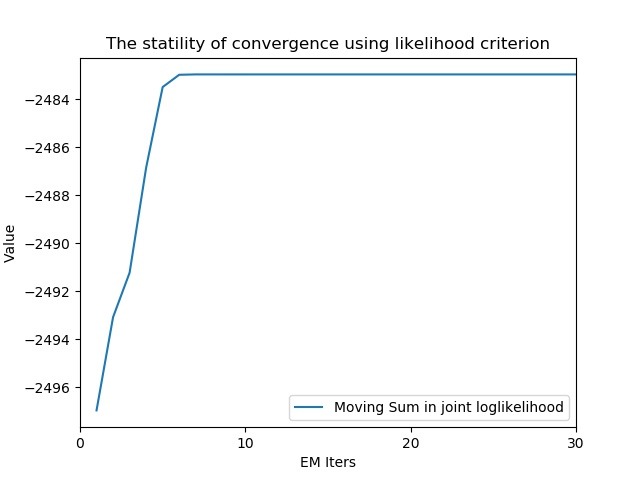
\includegraphics[width=.4\textwidth]{value_W=20_ll.jpg}
}
\subfigure{
{(b)}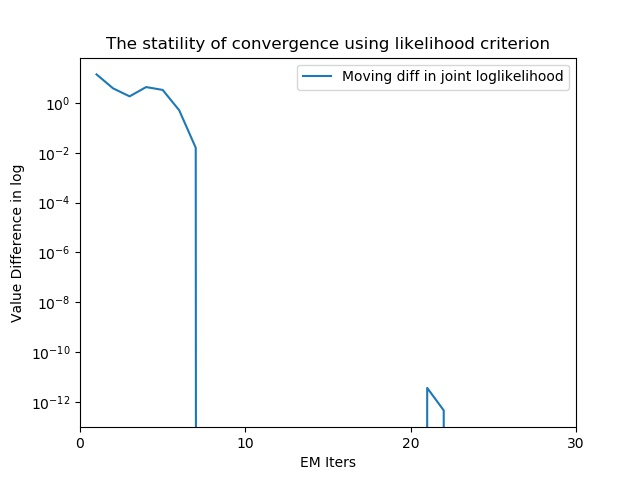
\includegraphics[width=.4\textwidth]{value_diff_W=20_ll.jpg}
}
\subfigure{
{(c)}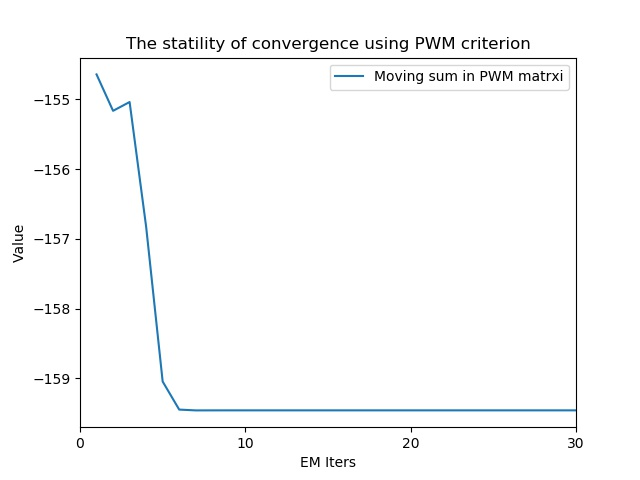
\includegraphics[width=.4\textwidth]{value_W=20_pwm.jpg}
}
\subfigure{
{(d)}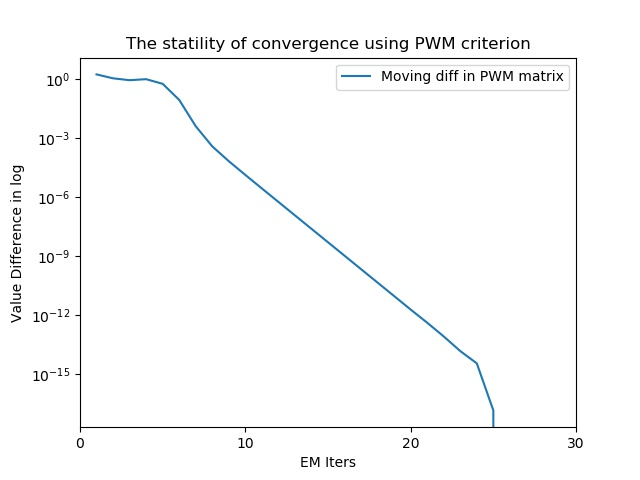
\includegraphics[width=.4\textwidth]{value_diff_W=20_pwm.jpg}
}
\caption{Comparison between EM convergence criterion. (a) the log likelihood value till convergence (b) the log likelihood moving difference  (c) the sum of PWM till convergence (d) the moving difference of PWM matrix. The discontinuity in (b) indicates the numerical instability and the converged state is indeed fluctuating despite the apparent smoothness in (a)  }

\end{figure}




\begin{table}
\setlength\tabcolsep{4pt} % default value is 6pt
\footnotesize
\centering
  \caption{MEME model results for the synthetic toy dataset. Running MEME OOPS model for 2 passes with width range from 5 to 10}
  \label{sample2}

\begin{tabular}{cccccccccc}
  \multicolumn{10}{|c|}{\textbf{MEME PASS 1}}\\
   \hline
\toprule
 ID &  Name & Pred Sites &  Width & True Sites & True Width &  Loglihood &   P\_value &  Precision &  Recall \\
\midrule
          1 &          seq1 &     TAATCC &          6 &             TAATCC &          6 &    -26.791 &  0.000091 &       1.0 &     1.0 \\
          2 &          seq2 &     TAATCC &          6 &             TAATCC &          6 &    -26.579 &  0.000091 &       1.0 &     1.0 \\
          3 &          seq3 &     TAATCC &          6 &             TAATCC &          6 &    -27.211 &  0.000091 &       1.0 &     1.0 \\
          4 &          seq4 &     TAATCC &          6 &             TAATCC &          6 &    -27.841 &  0.000091 &       1.0 &     1.0 \\
          5 &          seq5 &     TAATCC &          6 &             TAATCC &          6 &    -28.056 &  0.000091 &       1.0 &     1.0 \\
          6 &          seq6 &     TAATCC &          6 &             TAATCC &          6 &    -28.266 &  0.000091 &       1.0 &     1.0 \\
          7 &          seq7 &     TAATCC &          6 &             TAATCC &          6 &    -28.048 &  0.000091 &       1.0 &     1.0 \\
          8 &          seq8 &     TAATCC &          6 &             TAATCC &          6 &    -28.472 &  0.000091 &       1.0 &     1.0 \\
          9 &          seq9 &     TAATCC &          6 &             TAATCC &          6 &    -29.102 &  0.000091 &       1.0 &     1.0 \\
         10 &         seq10 &     TAATCC &          6 &             TAATCC &          6 &    -28.051 &  0.000091 &       1.0 &     1.0 \\

   \hline
   \multicolumn{3}{c|}{Roc}& \multicolumn{3}{|c|}{Acc}& \multicolumn{2}{|c|}{Avg Char Precision}& \multicolumn{2}{|c}{Avg Char Recall}\\
    \hline
    \multicolumn{3}{c|}{1.0}&\multicolumn{3}{|c|}{1.0}&\multicolumn{2}{
    c|}{1.0}&\multicolumn{2}{|c|}{1.0}\\
   \hline
   \multicolumn{5}{c|}{\textbf{Consensus motif}}&     \multicolumn{5}{|c}{\textbf{TAAACC}}\\
 
\bottomrule
\end{tabular}
\begin{figure}[H]
\centering
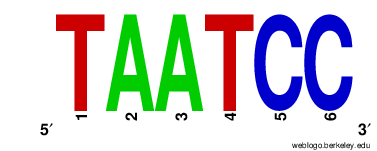
\includegraphics[scale=0.25]{test1.png}
\label{fig:svd}
\end{figure}
\centering
\begin{tabular}{cccccccccc}
  \multicolumn{10}{|c|}{\textbf{MEME PASS 2}}\\
   \hline
\toprule
 ID &   Name & Pred Sites & Width & True Sites & True Width &  Loglihood &   P\_value &  Precsion &    Recall \\
\midrule
  1 &   seq1 &     TAAAGC &     6 &     GAATCA &          6 &    -28.372 &  0.000765 &  1.000000 &  1.000000 \\
  2 &   seq2 &     AGAATC &     6 &     TAATCC &          6 &    -31.550 &  0.043653 &  1.000000 &  1.000000 \\
  3 &   seq3 &     TAATTA &     6 &     GAATCA &          6 &    -34.559 &  0.72000 &  1.000000 &  1.000000 \\
  4 &   seq4 &     TGAATC &     6 &     GAATCA &          6 &    -31.125 &  0.003950 &  0.833333 &  0.833333 \\
  5 &   seq5 &     TAATCC &     6 &     TAATCC &          6 &    -33.084 &  0.009714 &  1.000000 &  1.000000 \\
  6 &   seq6 &     TATACG &     6 &     GAATCA &          6 &    -35.450 &  0.142282 &  1.000000 &  1.000000 \\
  7 &   seq7 &     TAAACC &     6 &     TAATCC &          6 &    -28.884 &  0.000663 &  1.000000 &  1.000000 \\
  8 &   seq8 &     TGAATG &     6 &     TAATCC &          6 &    -33.967 &  0.040793 &  0.833333 &  0.833333 \\
  9 &   seq9 &     TAAACC &     6 &     GAATCA &          6 &    -30.695 &  0.000663 &  1.000000 &  1.000000 \\
 10 &  seq10 &     TGTAAC &     6 &     TAATCC &          6 &    -34.973 &  0.300210 &  0.500000 &  0.500000 \\
 
    \hline
   \multicolumn{3}{c|}{Roc}& \multicolumn{3}{|c|}{Acc}& \multicolumn{2}{|c|}{Avg Char Precision}& \multicolumn{2}{|c}{Avg Char Recall}\\
    \hline
    \multicolumn{3}{c|}{0.942}&\multicolumn{3}{|c|}{0.9}&\multicolumn{2}{
    c|}{0.9167}&\multicolumn{2}{|c|}{0.9167}\\
   \hline
   \multicolumn{5}{c|}{\textbf{Consensus motif}}&     \multicolumn{5}{|c}{\textbf{TAATCC}}\\
\bottomrule
\end{tabular}
\begin{figure}[H]
\centering
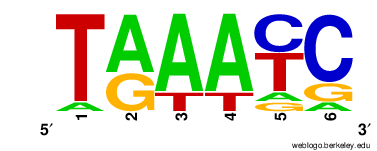
\includegraphics[scale=0.25]{test2.png}
\label{fig:svd}
\end{figure}
\end{table}


\begin{table}
\setlength\tabcolsep{0.5pt} % default value is 6pt
\footnotesize
  \caption{MEME model results for the crp dataset. Running MEME OOPS model for 2 passes with width range from 15 to 25}
  \label{sample2}
\centering
\begin{tabular}{c|c|c|c|c|c|c|c|c|c}
\multicolumn{10}{|c|}{\textbf{MEME PASS 1}}\\
   \hline
\toprule
 ID &     Name &         Pred Sites & Width &            True Sites & True Width &  Loglihood &   P\_value &  Precsion &  Recall \\
\midrule
 1 &    ce1cg &  TTGTGCTGGTTTTTGTGGC &    19 &  TTTTGTGGCATCGGGCGAGA &         20 &   -136.626 &  0.000085 &     0.474 &    0.45 \\
  2 &      ara &  AAGTGTCTATAATCACGGC &    19 &  AAAAGTGTCTATAATCACGG &         20 &   -143.498 &  0.02300 &     0.947 &    0.90 \\
  3 &    bglr1 &  ATTACACAAAGTTAATAAC &    19 &  AACTGTGAGCATGGTCATAT &         20 &   -130.171 &  0.000868 &     0.158 &    0.15 \\
  4 &      crp &  CATTGATGTACTGCATGTA &    19 &  GTATGCAAAGGACGTCACAT &         20 &   -138.536 &  0.000815 &     0.211 &    0.20 \\
  5 &      cya &  TTTAGACCATTTTTTCGTC &    19 &  AGGTGTTAAATTGATCACGT &         20 &   -135.530 &  0.000142 &     0.158 &    0.15 \\
  6 &    deop2 &  TTGTGATGTGTATCGAAGT &    19 &  AATTGTGATGTGTATCGAAG &         20 &   -132.696 &  0.000062 &     0.947 &    0.90 \\
  7 &     gale &  ATGTCACACTTTTCGCATC &    19 &  TAATTTATTCCATGTCACAC &         20 &   -135.954 &  0.000643 &     0.474 &    0.45 \\
  8 &      ilv &  TTTTCCCTTTGCTGAAAAA &    19 &  AAACGTGATCAACCCCTCAA &         20 &   -139.193 &  0.000433 &     0.211 &    0.20 \\
  9 &      lac &  GTGTGGAATTGTGAGCGGA &    19 &  GAATTGTGAGCGGATAACAA &         20 &   -137.148 &  0.000051 &     0.737 &    0.70 \\
 10 &     male &  TAGGGGCAAGGAGGATGGA &    19 &  TTCTGTAACAGAGATCACAC &         20 &   -139.853 &  0.000209 &     0.158 &    0.15 \\
 11 &     malk &  TCGTGATGTTGCTTGCAAA &    19 &  TTTCGTGATGTTGCTTGCAA &         20 &   -140.019 &  0.000271 &     0.947 &    0.90 \\
 12 &     malt &  TTTAGGTGAGTTGTTAATA &    19 &  AATTGTGACACAGTGCAAAT &         20 &   -135.605 &  0.000690 &     0.211 &    0.20 \\
 13 &     ompa &  ATTAAACATACCTTATACA &    19 &  ATGCCTGACGGAGTTCACAC &         20 &   -140.968 &  0.253923 &     0.158 &    0.15 \\
 14 &     tnaa &  ATTTAATATTGCTCCCCGA &    19 &  GATTGTGATTCGATTCACAT &         20 &   -128.842 &  0.000110 &     0.211 &    0.20 \\
 15 &     uxu1 &  GATTGACATGTCTTACCAA &    19 &  TGTTGTGATGTGGTTAACCC &         20 &   -136.058 &  0.000051 &     0.211 &    0.20 \\
 16 &   pbr322 &  TATGCGGCATCAGAGCAGA &    19 &  CGGTGTGAAATACCGCACAG &         20 &   -148.786 &  0.001040 &     0.158 &    0.15 \\
 17 &  trn9cat &  ATGAGACGTTGATCGGCAC &    19 &  AAATGAGACGTTGATCGGCA &         20 &   -139.082 &  0.000022 &     0.947 &    0.90 \\
 18 &      tdc &  TTGTGAGTGGTCGCACATA &    19 &  ATTTGTGAGTGGTCGCACAT &         20 &   -133.910 &  0.007082 &     0.947 &    0.90 \\
\bottomrule
  \hline
   \multicolumn{3}{c|}{Roc}& \multicolumn{3}{|c|}{Acc}& \multicolumn{2}{|c|}{Avg Char Precision}& \multicolumn{2}{|c}{Avg Char Recall}\\
    \hline
    \multicolumn{3}{c|}{0.942}&\multicolumn{3}{|c|}{0.889}&\multicolumn{2}{
    c|}{0.935}&\multicolumn{2}{|c|}{0.794}\\
   \hline
   \multicolumn{5}{c|}{\textbf{Consensus motif}}&     \multicolumn{5}{|c}{\textbf{TTTTGACATTGTTCACGGA}}\\

\end{tabular}

 \begin{figure}[H]
\centering
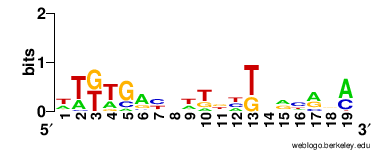
\includegraphics[scale=0.8]{crp2.png}
\label{fig:svd}
\end{figure}
\begin{tabular}{c|c|c|c|c|c|c|c|c|c}
\multicolumn{10}{|c|}{\textbf{MEME PASS 2}}\\
   \hline

\toprule
 ID &     Name &         Pred Sites & Width &            Matched Sites & True Width &  Loglihood &   P\_value &  Precsion &  Recall \\
\midrule
   1 &    ce1cg &  TGGTGTGAAAGACTGTT &    17 &  TTTTTTGATCGTTTTCACAA &         20 &   -136.679 &  0.000156 &     0.235 &    0.20 \\
  2 &      ara &  TGCTATGCCATAGCATT &    17 &  TTATTTGCACGGCGTCACAC &         20 &   -136.147 &  0.000124 &     0.235 &    0.20 \\
  3 &    bglr1 &  TGTTATATATAACTTTA &    17 &  AACTGTGAGCATGGTCATAT &         20 &   -128.485 &  0.000126 &     0.235 &    0.20 \\
  4 &      crp &  TACCGTGCAGTACAGTT &    17 &  GTATGCAAAGGACGTCACAT &         20 &   -135.690 &  0.000036 &     0.235 &    0.20 \\
  5 &      cya &  TAGCGCATCTTTCTTTA &    17 &  AGGTGTTAAATTGATCACGT &         20 &   -136.573 &  0.000360 &     0.176 &    0.15 \\
  6 &    deop2 &  TGTTGCGGAGTAGATGT &    17 &  AATTGTGATGTGTATCGAAG &         20 &   -134.485 &  0.000766 &     0.294 &    0.25 \\
  7 &     gale &  TTCCATGTCACACTTTT &    17 &  TAATTTATTCCATGTCACAC &         20 &   -135.983 &  0.000420 &     0.765 &    0.65 \\
  8 &      ilv &  TGTCTCCCCTGTAAAGC &    17 &  AAACGTGATCAACCCCTCAA &         20 &   -146.386 &  0.01340 &     0.294 &    0.25 \\
  9 &      lac &  AGGCACCCCAGGCTTTA &    17 &  TAATGTGAGTTAGCTCACTC &         20 &   -137.331 &  0.000053 &     0.176 &    0.15 \\
 10 &     male &  TGCCGTATAAAGAAACT &    17 &  TTCTGTAACAGAGATCACAC &         20 &   -140.381 &  0.000508 &     0.176 &    0.15 \\
 11 &     malk &  GGTCATGTAAGGAATTT &    17 &  TTTCGTGATGTTGCTTGCAA &         20 &   -137.976 &  0.000058 &     0.235 &    0.20 \\
 12 &     malt &  CGTCATCGCTTGCATTA &    17 &  AATTGTGACACAGTGCAAAT &         20 &   -131.848 &  0.000017 &     0.235 &    0.20 \\
 13 &     ompa &  CCTTATACAAGACTTTT &    17 &  ATGCCTGACGGAGTTCACAC &         20 &   -133.944 &  0.000061 &     0.176 &    0.15 \\
 14 &     tnaa &  TTTTAAACATTAAAATT &    17 &  GATTGTGATTCGATTCACAT &         20 &   -134.021 &  0.024075 &     0.235 &    0.20 \\
 15 &     uxu1 &  CGCCATCTCATCCGATG &    17 &  TGTTGTGATGTGGTTAACCC &         20 &   -137.875 &  0.000329 &     0.235 &    0.20 \\
 16 &   pbr322 &  TACCGCATCAGGCGCTC &    17 &  CGGTGTGAAATACCGCACAG &         20 &   -141.649 &  0.000343 &     0.412 &    0.35 \\
 17 &  trn9cat &  CTTCGCAGAATAAATAA &    17 &  CTGTGACGGAAGATCACTTC &         20 &   -143.591 &  0.002621 &     0.235 &    0.20 \\
 18 &      tdc &  GGTCGCACATATCCTGT &    17 &  ATTTGTGAGTGGTCGCACAT &         20 &   -134.064 &  0.013375 &     0.588 &    0.50 \\
\bottomrule
  \hline
   \multicolumn{3}{c|}{Roc}& \multicolumn{3}{|c|}{Acc}& \multicolumn{2}{|c|}{Avg Char Precision}& \multicolumn{2}{|c}{Avg Char Recall}\\
    \hline
    \multicolumn{3}{c|}{0.356}&\multicolumn{3}{|c|}{ 0.055}&\multicolumn{2}{
    c|}{0.288}&\multicolumn{2}{|c|}{0.244}\\
   \hline
   \multicolumn{5}{c|}{\textbf{Consensus motif}}&     \multicolumn{5}{|c}{\textbf{TGTGATCGAGTTCACAT}}\\ 
 
\bottomrule
\end{tabular}

 \begin{figure}[H]
\centering
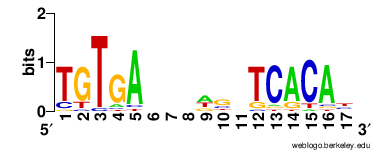
\includegraphics[scale=0.8]{crp_1.png}
\label{fig:svd}
\end{figure}
\end{table}








\begin{table}
\setlength\tabcolsep{0.5pt} % default value is 6pt
\footnotesize
  \caption{MEME model results for the lex dataset. Running MEME ZOOPS model for 2 passes with width range from 15 to 25}
  \label{sample2}
\centering
\begin{tabular}{c|c|c|c|c|c|c|c|c|c}
\multicolumn{10}{|c|}{\textbf{MEME PASS 1}}\\
   \hline
\toprule
 ID &     Name &         Pred Sites & Width &            Matched Sites & True Width &  Loglihood &   P\_value &  Precsion &  Recall \\
\midrule
 1 &  cloacin-df13 &  TACTGTGTATATATACA &    17 &  TACTGTGTATATATACAGTA &         20 &  -256.804 &        0 &        1 &   0.85 \\
  2 &    colicin-e1 &  TGCTGTATATAAAACCA &    17 &  TGCTGTATATAAAACCAGTG &         20 &  -255.396 &        0 &        1 &   0.85 \\
  3 &    colicin-ia &  TACTGTATATGTATCCA &    17 &  TACTGTATATGTATCCATAT &         20 &  -254.668 &        0 &        1 &   0.85 \\
  4 &    colicin-ib &  TACTGTATATGTATCCA &    17 &  TACTGTATATGTATCCATAT &         20 &  -253.844 &        0 &        1 &   0.85 \\
  5 &          reca &  TACTGTATGAGCATACA &    17 &  TACTGTATGAGCATACAGTA &         20 &  -263.206 &    2e-07 &        1 &   0.85 \\
  6 &          recn &  TACTGTATATAAAACCA &    17 &  TACTGTATATAAAACCAGTT &         20 &  -254.504 &        0 &        1 &   0.85 \\
  7 &          sula &  TACTGTACATCCATACA &    17 &  TACTGTACATCCATACAGTA &         20 &   -261.79 &    1e-07 &        1 &   0.85 \\
  8 &    umu-operon &  TACTGTATATAAAAACA &    17 &  TACTGTATATAAAAACAGTA &         20 &  -256.146 &        0 &        1 &   0.85 \\
  9 &          uvra &  TACTGTATATTCATTCA &    17 &  TACTGTATATTCATTCAGGT &         20 &   -262.44 &        0 &        1 &   0.85 \\
 10 &          uvrb &  AACTGTTTTTTTATCCA &    17 &  AACTGTTTTTTTATCCAGTA &         20 &  -261.888 &  2.2e-06 &        1 &   0.85 \\
 11 &          uvrd &  ATCTGTATATATACCCA &    17 &  ATCTGTATATATACCCAGCT &         20 &  -266.116 &    1e-07 &        1 &   0.85 \\
 12 &     colicin-a &  TACTGTATATAAACACA &    17 &  TACTGTATATAAACACATGT &         20 &  -171.027 &        0 &        1 &   0.85 \\
 13 &          lexA &  AACTGTATATACACCCA &    17 &  AACTGTATATACACCCAGGG &         20 &  -221.896 &        0 &        1 &   0.85 \\
 14 &    muc-operon &  TACTGTATAAATAAACA &    17 &  TACTGTATAAATAAACAGTT &         20 &  -200.753 &        0 &        1 &   0.85 \\
 15 &          hima &                N/A &   N/A &                   N/A &        N/A &       N/A &      N/A &      N/A &    N/A \\
 16 &          uvrc &                N/A &   N/A &                   N/A &        N/A &       N/A &      N/A &      N/A &    N/A \\
\bottomrule
  \hline
   \multicolumn{3}{c|}{Roc}& \multicolumn{3}{|c|}{Acc}& \multicolumn{2}{|c|}{Avg Char Precision}& \multicolumn{2}{|c}{Avg Char Recall}\\
    \hline
    \multicolumn{3}{c|}{1.0}&\multicolumn{3}{|c|}{1.0}&\multicolumn{2}{
    c|}{1.0}&\multicolumn{2}{|c|}{0.850}\\
   \hline
   \multicolumn{5}{c|}{\textbf{Consensus motif}}&     \multicolumn{5}{|c}{\textbf{TACTGTATATATATCCA}}\\

\end{tabular}

 \begin{figure}[H]
\centering
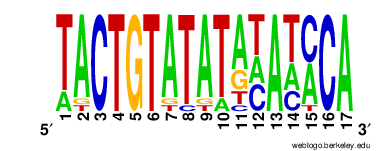
\includegraphics[scale=0.8]{lex1.png}
\label{fig:svd}
\end{figure}
\begin{tabular}{c|c|c|c|c|c|c|c|c|c}
\multicolumn{10}{|c|}{\textbf{MEME PASS 2}}\\
   \hline

\toprule
 ID &     Name &         Pred Sites & Width &            Matched Sites & True Width &  Loglihood &   P\_value &  Precsion &  Recall \\
\midrule
   1 &  cloacin-df13 &                N/A &   N/A &                   N/A &        N/A &       N/A &      N/A &      N/A &    N/A \\
  2 &    colicin-e1 &                N/A &   N/A &                   N/A &        N/A &       N/A &      N/A &      N/A &    N/A \\
  3 &    colicin-ia &                N/A &   N/A &                   N/A &        N/A &       N/A &      N/A &      N/A &    N/A \\
  4 &    colicin-ib &                N/A &   N/A &                   N/A &        N/A &       N/A &      N/A &      N/A &    N/A \\
  5 &          reca &  TACTGCGTATGCTTGCA &    17 &  TACTGTATGAGCATACAGTA &         20 &  -264.034 &    4e-07 &    0.294 &   0.25 \\
  6 &          recn &                N/A &   N/A &                   N/A &        N/A &       N/A &      N/A &      N/A &    N/A \\
  7 &          sula &                N/A &   N/A &                   N/A &        N/A &       N/A &      N/A &      N/A &    N/A \\
  8 &    umu-operon &                N/A &   N/A &                   N/A &        N/A &       N/A &      N/A &      N/A &    N/A \\
  9 &          uvra &                N/A &   N/A &                   N/A &        N/A &       N/A &      N/A &      N/A &    N/A \\
 10 &          uvrb &                N/A &   N/A &                   N/A &        N/A &       N/A &      N/A &      N/A &    N/A \\
 11 &          uvrd &                N/A &   N/A &                   N/A &        N/A &       N/A &      N/A &      N/A &    N/A \\
 12 &     colicin-a &                N/A &   N/A &                   N/A &        N/A &       N/A &      N/A &      N/A &    N/A \\
 13 &          lexA &  TGCTGTATATACTCACA &    17 &  TGCTGTATATACTCACAGCA &         20 &  -225.431 &    3e-07 &        1 &   0.85 \\
 14 &    muc-operon &                N/A &   N/A &                   N/A &        N/A &       N/A &      N/A &      N/A &    N/A \\
 15 &          hima &  AAATGTGTAGAGGCATT &    17 &                   N/A &        N/A &  -268.236 &  2.3e-06 &        0 &      0 \\
 16 &          uvrc &  AACGGTGAACAGCTACC &    17 &                   N/A &        N/A &  -263.294 &    8e-07 &        0 &      0 \\
\bottomrule
  \hline
   \multicolumn{3}{c|}{Roc}& \multicolumn{3}{|c|}{Acc}& \multicolumn{2}{|c|}{Avg Char Precision}& \multicolumn{2}{|c}{Avg Char Recall}\\
    \hline
    \multicolumn{3}{c|}{0.510}&\multicolumn{3}{|c|}{ 0.0625}&\multicolumn{2}{
    c|}{0.323}&\multicolumn{2}{|c|}{0.275}\\
   \hline
   \multicolumn{5}{c|}{\textbf{Consensus motif}}&     \multicolumn{5}{|c}{\textbf{AACTGTGTATAGTTACA}}\\ 
 
\bottomrule
\end{tabular}

 \begin{figure}[H]
\centering
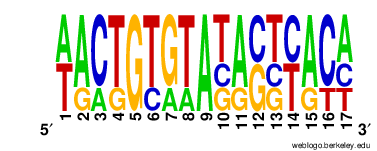
\includegraphics[scale=0.8]{lex2.png}
\label{fig:svd}
\end{figure}
\end{table}



\begin{table}
\setlength\tabcolsep{30pt} % default value is 6pt

  \caption{MEME model results for the crplex dataset. Running MEME ZOOPS model for 3 passes with width range from 15 to 25}
  \label{sample2}
\centering
\scalebox{0.45}{
\begin{tabular}{c|c|c|c|c|c|c|c|c|c}
\multicolumn{10}{|c|}{\textbf{MEME PASS 1}}\\
   \hline
\toprule
 ID &     Name &         Pred Sites & Width &            Matched Sites & True Width &  Loglihood &   P\_value &  Precsion &  Recall \\
\midrule
1 &         ce1cg &                 N/A &   N/A &                   N/A &        N/A &       N/A &        N/A &      N/A &    N/A \\
  2 &           ara &  AAAGTGTCTATAATCACG &    18 &  AAAAGTGTCTATAATCACGG &         20 &  -135.837 &   9.04e-05 &        1 &    0.9 \\
  3 &         bglr1 &  TAACTTTATAAATTCCTA &    18 &  AACTGTGAGCATGGTCATAT &         20 &  -129.999 &   6.74e-05 &    0.222 &    0.2 \\
  4 &           crp &                 N/A &   N/A &                   N/A &        N/A &       N/A &        N/A &      N/A &    N/A \\
  5 &           cya &                 N/A &   N/A &                   N/A &        N/A &       N/A &        N/A &      N/A &    N/A \\
  6 &         deop2 &                 N/A &   N/A &                   N/A &        N/A &       N/A &        N/A &      N/A &    N/A \\
  7 &          gale &  CTTGTGTAAACGATTCCA &    18 &  TAATTTATTCCATGTCACAC &         20 &   -133.79 &   3.15e-05 &    0.333 &    0.3 \\
  8 &           ilv &  TTGCTGAAAAATTTTCCA &    18 &  AAACGTGATCAACCCCTCAA &         20 &  -137.987 &  0.0001674 &    0.167 &   0.15 \\
  9 &           lac &                 N/A &   N/A &                   N/A &        N/A &       N/A &        N/A &      N/A &    N/A \\
 10 &          male &                 N/A &   N/A &                   N/A &        N/A &       N/A &        N/A &      N/A &    N/A \\
 11 &          malk &  CTTCTGTGAACTAAACCG &    18 &  TTCTGTGAACTAAACCGAGG &         20 &  -137.879 &   9.25e-05 &    0.944 &   0.85 \\
 12 &          malt &  ACAGTGCAAATTCAGACA &    18 &  AATTGTGACACAGTGCAAAT &         20 &  -135.514 &  0.0003658 &    0.611 &   0.55 \\
 13 &          ompa &  ATACCTTATACAAGACTT &    18 &  ATGCCTGACGGAGTTCACAC &         20 &  -138.158 &  0.0038609 &    0.167 &   0.15 \\
 14 &          tnaa &  AATCTTTAAAAAAAGCAT &    18 &  GATTGTGATTCGATTCACAT &         20 &  -134.174 &  0.0035259 &    0.167 &   0.15 \\
 15 &          uxu1 &                 N/A &   N/A &                   N/A &        N/A &       N/A &        N/A &      N/A &    N/A \\
 16 &        pbr322 &                 N/A &   N/A &                   N/A &        N/A &       N/A &        N/A &      N/A &    N/A \\
 17 &       trn9cat &                 N/A &   N/A &                   N/A &        N/A &       N/A &        N/A &      N/A &    N/A \\
 18 &           tdc &                 N/A &   N/A &                   N/A &        N/A &       N/A &        N/A &      N/A &    N/A \\
 19 &  cloacin-df13 &  ATACTGTGTATATATACA &    18 &  TACTGTGTATATATACAGTA &         20 &  -257.849 &      1e-07 &    0.944 &   0.85 \\
 20 &    colicin-e1 &  ATGCTGTATATAAAACCA &    18 &  TGCTGTATATAAAACCAGTG &         20 &  -254.646 &          0 &    0.944 &   0.85 \\
 21 &    colicin-ia &  ATACTGTATATGTATCCA &    18 &  TACTGTATATGTATCCATAT &         20 &  -256.138 &          0 &    0.944 &   0.85 \\
 22 &    colicin-ib &  GTACTGTATATGTATCCA &    18 &  TACTGTATATGTATCCATAT &         20 &  -256.461 &      1e-07 &    0.944 &   0.85 \\
 23 &          reca &  ATACTGTATGAGCATACA &    18 &  TACTGTATGAGCATACAGTA &         20 &  -265.504 &    1.4e-06 &    0.944 &   0.85 \\
 24 &          recn &  TTACTGTATATAAAACCA &    18 &  TACTGTATATAAAACCAGTT &         20 &  -255.715 &          0 &    0.944 &   0.85 \\
 25 &          sula &  GTACTGTACATCCATACA &    18 &  TACTGTACATCCATACAGTA &         20 &  -265.321 &    4.7e-06 &    0.944 &   0.85 \\
 26 &    umu-operon &  CTACTGTATATAAAAACA &    18 &  TACTGTATATAAAAACAGTA &         20 &  -258.049 &          0 &    0.944 &   0.85 \\
 27 &          uvra &  ATACTGTATATTCATTCA &    18 &  TACTGTATATTCATTCAGGT &         20 &  -265.279 &      4e-07 &    0.944 &   0.85 \\
 28 &          uvrb &                 N/A &   N/A &                   N/A &        N/A &       N/A &        N/A &      N/A &    N/A \\
 29 &          uvrd &  AATCTGTATATATACCCA &    18 &  ATCTGTATATATACCCAGCT &         20 &  -267.195 &      1e-07 &    0.944 &   0.85 \\
 30 &     colicin-a &  TTACTGTATATAAACACA &    18 &  TACTGTATATAAACACATGT &         20 &  -173.226 &          0 &    0.944 &   0.85 \\
 31 &          lexA &  TAACTGTATATACACCCA &    18 &  AACTGTATATACACCCAGGG &         20 &  -223.832 &      1e-07 &    0.944 &   0.85 \\
 32 &    muc-operon &  ATACTGTATAAATAAACA &    18 &  TACTGTATAAATAAACAGTT &         20 &  -201.866 &      1e-07 &    0.944 &   0.85 \\
 33 &          hima &                 N/A &   N/A &                   N/A &        N/A &       N/A &        N/A &      N/A &    N/A \\
 34 &          uvrc &                 N/A &   N/A &                   N/A &        N/A &       N/A &        N/A &      N/A &    N/A \\
\bottomrule
  \hline
   \multicolumn{3}{c|}{Roc}& \multicolumn{3}{|c|}{Acc}& \multicolumn{2}{|c|}{Avg Char Precision}& \multicolumn{2}{|c}{Avg Char Recall}\\
    \hline
    \multicolumn{3}{c|}{0.747}&\multicolumn{3}{|c|}{ 0.5}&\multicolumn{2}{
    c|}{0.756}&\multicolumn{2}{|c|}{0.680}\\
   \hline
   \multicolumn{5}{c|}{\textbf{Consensus motif}}&     \multicolumn{5}{|c}{\textbf{ATACTGTATATAAATCCA}}\\

\end{tabular}}

\scalebox{0.45}{
\begin{tabular}{c|c|c|c|c|c|c|c|c|c}
\multicolumn{10}{|c|}{\textbf{MEME PASS 2}}\\
   \hline
\toprule
 ID &     Name &         Pred Sites & Width &            Matched Sites & True Width &  Loglihood &   P\_value &  Precsion &  Recall \\
\midrule
1 &         ce1cg &  TTTTTTGATCGTTTTCACA &    19 &  TTTTTTGATCGTTTTCACAA &         20 &  -131.232 &      2e-07 &        1 &   0.95 \\
  2 &           ara &  TTATTTGCACGGCGTCACA &    19 &  TTATTTGCACGGCGTCACAC &         20 &  -131.181 &    1.1e-06 &        1 &   0.95 \\
  3 &         bglr1 &  AACTGTGAGCATGGTCATA &    19 &  AACTGTGAGCATGGTCATAT &         20 &  -129.676 &  0.0001454 &        1 &   0.95 \\
  4 &           crp &  GTATGCAAAGGACGTCACA &    19 &  GTATGCAAAGGACGTCACAT &         20 &  -134.921 &   2.54e-05 &        1 &   0.95 \\
  5 &           cya &  TTCTTTACGGTCAATCAGC &    19 &  AGGTGTTAAATTGATCACGT &         20 &  -137.404 &  0.0008412 &    0.211 &    0.2 \\
  6 &         deop2 &  TTATTTGAACCAGATCGCA &    19 &  TTATTTGAACCAGATCGCAT &         20 &  -130.854 &    4.6e-06 &        1 &   0.95 \\
  7 &          gale &  TAATTTATTCCATGTCACA &    19 &  TAATTTATTCCATGTCACAC &         20 &  -133.905 &   4.88e-05 &        1 &   0.95 \\
  8 &           ilv &                  N/A &   N/A &                   N/A &        N/A &       N/A &        N/A &      N/A &    N/A \\
  9 &           lac &  TAATGTGAGTTAGCTCACT &    19 &  TAATGTGAGTTAGCTCACTC &         20 &   -136.91 &   4.58e-05 &        1 &   0.95 \\
 10 &          male &  TTCTGTAACAGAGATCACA &    19 &  TTCTGTAACAGAGATCACAC &         20 &  -136.515 &   1.34e-05 &        1 &   0.95 \\
 11 &          malk &  TTTCGTGATGTTGCTTGCA &    19 &  TTTCGTGATGTTGCTTGCAA &         20 &  -138.612 &   9.17e-05 &        1 &   0.95 \\
 12 &          malt &                  N/A &   N/A &                   N/A &        N/A &       N/A &        N/A &      N/A &    N/A \\
 13 &          ompa &  ATGCCTGACGGAGTTCACA &    19 &  ATGCCTGACGGAGTTCACAC &         20 &  -133.145 &   2.84e-05 &        1 &   0.95 \\
 14 &          tnaa &  GATTGTGATTCGATTCACA &    19 &  GATTGTGATTCGATTCACAT &         20 &   -128.86 &   3.43e-05 &        1 &   0.95 \\
 15 &          uxu1 &  TGTTGTGATGTGGTTAACC &    19 &  TGTTGTGATGTGGTTAACCC &         20 &  -135.414 &   3.07e-05 &        1 &   0.95 \\
 16 &        pbr322 &  TTAACTATGCGGCATCAGA &    19 &  CGGTGTGAAATACCGCACAG &         20 &  -139.804 &   0.000127 &    0.158 &   0.15 \\
 17 &       trn9cat &  AAATGAGACGTTGATCGGC &    19 &  AAATGAGACGTTGATCGGCA &         20 &  -142.749 &  0.0024568 &        1 &   0.95 \\
 18 &           tdc &  ATTTGTGAGTGGTCGCACA &    19 &  ATTTGTGAGTGGTCGCACAT &         20 &   -128.57 &    6.1e-06 &        1 &   0.95 \\
 19 &  cloacin-df13 &                  N/A &   N/A &                   N/A &        N/A &       N/A &        N/A &      N/A &    N/A \\
 20 &    colicin-e1 &  TTTTTTGATCGTTTTCACA &    19 &  TGCTGTATATAAAACCAGTG &         20 &  -256.275 &      2e-07 &    0.158 &   0.15 \\
 21 &    colicin-ia &  CTTTCTGAACGGTGTAACA &    19 &  TACTGTATATGTATCCATAT &         20 &  -261.967 &   1.22e-05 &    0.211 &    0.2 \\
 22 &    colicin-ib &  CTTTCTGAACGGTATAACA &    19 &  TACTGTATATGTATCCATAT &         20 &  -260.862 &   1.23e-05 &    0.263 &   0.25 \\
 23 &          reca &                  N/A &   N/A &                   N/A &        N/A &       N/A &        N/A &      N/A &    N/A \\
 24 &          recn &                  N/A &   N/A &                   N/A &        N/A &       N/A &        N/A &      N/A &    N/A \\
 25 &          sula &                  N/A &   N/A &                   N/A &        N/A &       N/A &        N/A &      N/A &    N/A \\
 26 &    umu-operon &  TTTAGCGATCTTGTTCAGT &    19 &  TACTGTATATAAAAACAGTA &         20 &  -265.429 &  0.0001508 &    0.211 &    0.2 \\
 27 &          uvra &  GTTTGTGATCGCCGGTAGC &    19 &  TACTGTATATTCATTCAGGT &         20 &  -270.795 &  0.0001078 &    0.158 &   0.15 \\
 28 &          uvrb &  GAGTTTACGCTGTATCAGA &    19 &  AACTGTTTTTTTATCCAGTA &         20 &  -265.142 &  0.0001372 &    0.211 &    0.2 \\
 29 &          uvrd &  ATTTTTACGCGGCGGTGCC &    19 &  ATCTGTATATATACCCAGCT &         20 &   -276.28 &  0.0004143 &    0.158 &   0.15 \\
 30 &     colicin-a &  TTTGGTGTGGCAGAGCACT &    19 &  ACATGTGAATATATACAGTT &         20 &   -181.85 &  0.0002252 &    0.211 &    0.2 \\
 31 &          lexA &  GATCTCATCCGTGATCACA &    19 &  AACTGTATATACACCCAGGG &         20 &  -231.822 &  0.0001806 &    0.263 &   0.25 \\
 32 &    muc-operon &                  N/A &   N/A &                   N/A &        N/A &       N/A &        N/A &      N/A &    N/A \\
 33 &          hima &  ATCATTGAGGGATTGAACC &    19 &                   N/A &        N/A &  -274.204 &  0.0006522 &        0 &      0 \\
 34 &          uvrc &  GATTATGCTGATGATCACC &    19 &                   N/A &        N/A &  -268.646 &  0.0002013 &        0 &      0 \\
\bottomrule
  \hline
   \multicolumn{3}{c|}{Roc}& \multicolumn{3}{|c|}{Acc}& \multicolumn{2}{|c|}{Avg Char Precision}& \multicolumn{2}{|c}{Avg Char Recall}\\
    \hline
    \multicolumn{3}{c|}{0.692}&\multicolumn{3}{|c|}{ 0.411}&\multicolumn{2}{
    c|}{0.600}&\multicolumn{2}{|c|}{0.570}\\
   \hline
   \multicolumn{5}{c|}{\textbf{Consensus motif}}&     \multicolumn{5}{|c}{\textbf{TTTTGTGATCGGGATCACA}}\\
  
\end{tabular}}

 
\scalebox{0.45}{
\begin{tabular}{c|c|c|c|c|c|c|c|c|c}
\multicolumn{10}{|c|}{\textbf{MEME PASS 3}}\\
   \hline
\toprule
 ID &     Name &         Pred Sites & Width &            Matched Sites & True Width &  Loglihood &   P\_value &  Precsion &  Recall \\
\midrule
 1 &         ce1cg &                   N/A &   N/A &                   N/A &        N/A &       N/A &        N/A &      N/A &    N/A \\
  2 &           ara &                   N/A &   N/A &                   N/A &        N/A &       N/A &        N/A &      N/A &    N/A \\
  3 &         bglr1 &                   N/A &   N/A &                   N/A &        N/A &       N/A &        N/A &      N/A &    N/A \\
  4 &           crp &                   N/A &   N/A &                   N/A &        N/A &       N/A &        N/A &      N/A &    N/A \\
  5 &           cya &  GTTAAATTGATCACGTTTTA &    20 &  AGGTGTTAAATTGATCACGT &         20 &  -133.206 &      9e-06 &      0.8 &    0.8 \\
  6 &         deop2 &                   N/A &   N/A &                   N/A &        N/A &       N/A &        N/A &      N/A &    N/A \\
  7 &          gale &                   N/A &   N/A &                   N/A &        N/A &       N/A &        N/A &      N/A &    N/A \\
  8 &           ilv &  TTTTTTGTTATCTGCAATTC &    20 &  AAACGTGATCAACCCCTCAA &         20 &  -135.905 &   1.61e-05 &     0.15 &   0.15 \\
  9 &           lac &                   N/A &   N/A &                   N/A &        N/A &       N/A &        N/A &      N/A &    N/A \\
 10 &          male &                   N/A &   N/A &                   N/A &        N/A &       N/A &        N/A &      N/A &    N/A \\
 11 &          malk &                   N/A &   N/A &                   N/A &        N/A &       N/A &        N/A &      N/A &    N/A \\
 12 &          malt &  TTTTAGGTGAGTTGTTAATA &    20 &  AATTGTGACACAGTGCAAAT &         20 &  -134.916 &  0.0001869 &      0.2 &    0.2 \\
 13 &          ompa &                   N/A &   N/A &                   N/A &        N/A &       N/A &        N/A &      N/A &    N/A \\
 14 &          tnaa &                   N/A &   N/A &                   N/A &        N/A &       N/A &        N/A &      N/A &    N/A \\
 15 &          uxu1 &                   N/A &   N/A &                   N/A &        N/A &       N/A &        N/A &      N/A &    N/A \\
 16 &        pbr322 &                   N/A &   N/A &                   N/A &        N/A &       N/A &        N/A &      N/A &    N/A \\
 17 &       trn9cat &                   N/A &   N/A &                   N/A &        N/A &       N/A &        N/A &      N/A &    N/A \\
 18 &           tdc &  TTGATATTTAAAGGTATTTA &    20 &  ATTTGTGAGTGGTCGCACAT &         20 &  -130.787 &   3.82e-05 &      0.2 &    0.2 \\
 19 &  cloacin-df13 &                   N/A &   N/A &                   N/A &        N/A &       N/A &        N/A &      N/A &    N/A \\
 20 &    colicin-e1 &  GGTTATATGTACAGTATTTA &    20 &  CAGTGGTTATATGTACAGTA &         20 &  -257.495 &      6e-07 &      0.8 &    0.8 \\
 21 &    colicin-ia &                   N/A &   N/A &                   N/A &        N/A &       N/A &        N/A &      N/A &    N/A \\
 22 &    colicin-ib &                   N/A &   N/A &                   N/A &        N/A &       N/A &        N/A &      N/A &    N/A \\
 23 &          reca &  TATTGACTATCCGGTATTAC &    20 &  TACTGTATGAGCATACAGTA &         20 &  -267.268 &   1.13e-05 &      0.2 &    0.2 \\
 24 &          recn &  TTTATACTGTACACAATAAC &    20 &  TACTGTACACAATAACAGTA &         20 &  -260.574 &    4.5e-06 &      0.8 &    0.8 \\
 25 &          sula &                   N/A &   N/A &                   N/A &        N/A &       N/A &        N/A &      N/A &    N/A \\
 26 &    umu-operon &                   N/A &   N/A &                   N/A &        N/A &       N/A &        N/A &      N/A &    N/A \\
 27 &          uvra &                   N/A &   N/A &                   N/A &        N/A &       N/A &        N/A &      N/A &    N/A \\
 28 &          uvrb &  GTTTTTTTATCCAGTATAAT &    20 &  AACTGTTTTTTTATCCAGTA &         20 &  -262.377 &    6.3e-06 &      0.8 &    0.8 \\
 29 &          uvrd &                   N/A &   N/A &                   N/A &        N/A &       N/A &        N/A &      N/A &    N/A \\
 30 &     colicin-a &                   N/A &   N/A &                   N/A &        N/A &       N/A &        N/A &      N/A &    N/A \\
 31 &          lexA &  GGTTTATTGTGCAGTTTATG &    20 &  TGCTGTATATACTCACAGCA &         20 &  -227.066 &    1.4e-06 &     0.15 &   0.15 \\
 32 &    muc-operon &  TTTTATCTGCAAAGAATTTC &    20 &  TACTGTATAAATAAACAGTT &         20 &  -204.927 &    2.2e-06 &     0.15 &   0.15 \\
 33 &          hima &                   N/A &   N/A &                   N/A &        N/A &       N/A &        N/A &      N/A &    N/A \\
 34 &          uvrc &  GTTTGTCTGAACGTGAATTG &    20 &                   N/A &        N/A &  -265.468 &    8.2e-06 &        0 &      0 \\
\bottomrule
  \hline
   \multicolumn{3}{c|}{Roc}& \multicolumn{3}{|c|}{Acc}& \multicolumn{2}{|c|}{Avg Char Precision}& \multicolumn{2}{|c}{Avg Char Recall}\\
    \hline
    \multicolumn{3}{c|}{0.564}&\multicolumn{3}{|c|}{0.147}&\multicolumn{2}{
    c|}{0.386}&\multicolumn{2}{|c|}{0.386}\\
   \hline
   \multicolumn{5}{c|}{\textbf{Consensus motif}}&     \multicolumn{5}{|c}{\textbf{TTTTTATTGTACAGTATTTA}}\\

\end{tabular}}

 \begin{figure}[H]
\centering
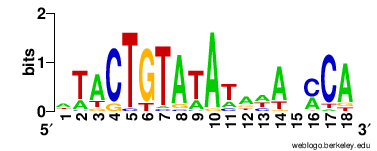
\includegraphics[scale=0.45]{crplex1.png}
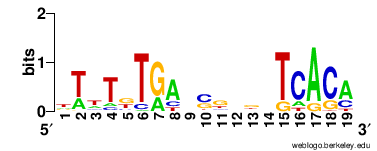
\includegraphics[scale=0.45]{crplex2.png}
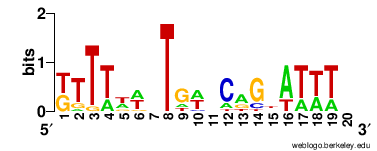
\includegraphics[scale=0.45]{crplex3.png}
\label{fig:svd}
\end{figure}
\end{table}




\begin{table}
\caption{The convergence evaluation obtained by  of 'TEST' algorithm. The result obtained by running the OOPs model for the crp data}
\centering
  \begin{tabular}{|c|c|c|}
    \textbf{Starting Subsequence}     & \textbf{Converged Consensus Sequence} &\textbf{Number of EM iterations till convergence}\\
  \midrule
TTTTGATCCTTTTCACA&TTGTGATATAGTTCACA&16\\

TGTGATCGATTTCACAA&TGTGATCGAGTTCACAT&14\\

TTTGTGATCGGTTTCACA&ATTGTGATTATTTTCACA&10\\

TTTGTGAACGTTTTCACA&TTTGTGAACGAGTTCACA&9\\
TTTGTGATCGTTTTCACA&TTTGTGAACGAGTTCACA&13\\
TTGTGATCGGTTTCACAAA&TTGTGAACGAGTTCACACA&25\\

TTTTTTGAACGATTTCACA&TTATGTGATCGAGCTCACA&14\\
TTTTTGTGATCGTGTTCAC&ATTTTGTGAATTGGCTCAC&11\\
TTGTGATCTTTTTCACAAA&TTGTGATCGAGTTCACACT&28\\
\hline
\end{tabular}
\end{table}






\begin{table}[ht]
\centering
 \caption{The precision and recall score change with respect to motif prior $\beta$. The best $\lambda$ value is around 0.02. The score is gathered at the second pass of the MEME by running a ZOOPS model on the crp dataset}
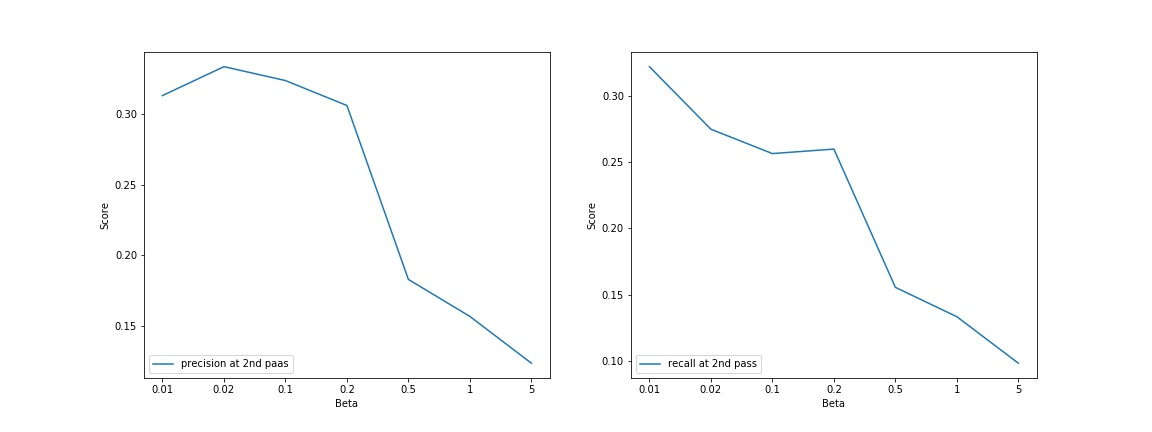
\includegraphics[scale=0.3]{lambda.jpg}
\label{fig:lambda}
\end{table}



\begin{table}
\caption{The convergence evaluation obtained by  of 'TEST' algorithm. The result obtained by running the OOPs model for the crp data}
\centering
  \begin{tabular}{|c|c|c|c|c|c|c|}
    \textbf{ data}     & \textbf{Number of added random sequences}&\textbf{ROC}&\textbf{Accuaray} &\textbf{Avg Precision}&\textbf{Avg Recall}\\
  \midrule
crp.fa & 0  &0.971     & 0.944   &    0.972    &   0.778 \\

crp5.fa & 5 & 0.963  &0.930 &  0.963 &0.771 \\


crp10.fa & 20 & 0.888  &0.883 & 0.828 &0.655 \\

crp20.fa & 10 & 0.920  &0.911 & 0.8744 &0.71 \\

crp30.fa & 30 & 0.852  &0.810 & 0.742 &0.624 \\

crp50.fa & 50 & 0.857  &0.749 & 0.7231 &0.695 \\

\hline
   
\end{tabular}
\end{table}
     


\section{Discussion}

From Figure 2, we can see that using the convergence criterion based on PWM is more stable than the loglikelihood since the moving difference does not show any sudden clip or discontinuity during the process till convergence. If we zoom in the curve in (a), the likelihood value is fluctuating while in theory there should not be any decrease during the convergence process, the transition between positive and negative moving difference explains the discontinuity in (b). 

The result of running OOPS model on the toy data set is shown in Table 4. The result of running OOPS model on crp dataset is shown in Table 5. The result of running ZOOPs model on lex and crplex are shown below as well in Table 5, Table 6 and Table 7 accordingly. Note that The OOPS model result is not shown here for the lex dataset and since the result of OOPS models is equivalent to the first pass of the ZOOPS model and its performance degrades at the second pass since it assumes every sequence must contain one motif. Also, ZOOPs model will be a better fit for these real data sets that have zero occurrence of motif for a sequence.

The OOPS model from Table 4 and 5 indicates a difficulty of this model generalizing to a real world dataset where there are more noise in the truth motif sets. One of result is that the predicted Width might always be different with the actual motif width though their difference is minor. The motif level precision and recall directly show the matching accuracy. Also, the likelihood and p value are very indicative of the strength of prediction. They could be used to estimate the preciseness during the inference stage when there is no label available to us. 

It could be seen that the ZOOPs model works well on the lex dataset since the first pass achieves exact match without a single mistake in Table 6. Although it does not find all the truth motifs at the second pass, the motif set it found during the second still share somewhat significant similarity among them based on the metrics.

The Table 7 evaluates the performance of ZOOPS model on the composite crplex dataset. It could be seen here with more inputs and more diverse mix of different motif, the performance of the MEME slightly degrades compared to the results obtained by running it on individual dataset.

This susceptibility to noise could also be observed in table 9, where I ran the same MEME model on the crp datasets that contain different number of random generated sequences. As the random sequence start to dominate, the performance of MEME is maintained at relatively the same level as the original data given the roc and accuracy is still around 0.9 and 0.8 correspondingly.

Additionally, the power of 'TEST' could be approved based on the results in Table 8. The converged sequence are close to the starting subsequences obtained by the 'TEST' algorithm. The number of EM iterations with test algorithm are all less than 50, meaning it significantly accelerates the speed of convergence. Although the 'TEST' algorithm introduces some extra running time before running the MEME, but this could be largely compensated with dynamic programming. 

Furthermore,from figure 3, the model is highly sensitive to the prior $\beta$ that incorporates knowledge about motif column at the second pass of the MEME, meaning some decent picks of prior will be critical for interpreting and predicting multiple motifs.

% MEME algorithm can discover motifs in a satisfactory time by a compromising strategy such as discarding a majority of the sequences but discarding data is far from ideal as it can decrease the chance of discovering motifs corresponding to infrequent cofactors

% There are two principal types of motif discovery algorithms; i.e. enumeration approach and probabilistic technique. Enumeration approach searches for consensus sequences; motifs are predicted based on the enumeration of words and computing word similarities so this appro

% https://www.ncbi.nlm.nih.gov/pmc/articles/PMC2648755/#B10

% In the early versions of MEME, the exact motif length are specified as one of its input parameters. At each pass f


% multiple start based on different width {W} and 


\section{Conclusion}
Overall, the modified MEME is powerful since all it requires from the user is just the input sequences and type of model should be ran on. The statistical width selection typically works well with small amount of allowable width shift. The ZOOPS model is impressive in terms of generalization performance since the predictive power is able to be maintained as more noisy inputs are added. The prior information is useful and it allows user to incorporate prior knowledge to help with better convergence. Overall, the distinct drawback of using this version of MEME its slow executing speed since we will be running the 'TEST' algorithm across the entire dataset and MEME are testing a bunch of different width and $lambda$ to determine the best set of parameters for a given sequences. However, those computations are highly parallel and this algorithm could be extended and accelerated in cloud computing environment where multiple machines could be running simultaneously. 


\section{References}
[1] Timothy L. Bailey and Charles Elkan, “Fitting a mixture model by expectation maximization to discover motifs in biopolymers”, Proceedings of the Second International Conference on Intelligent Systems for Molecular Biology (ISMB’94), pp. 28–36, AAAI Press, Menlo Park, California, August, 1994.

[2] Timothy L. Bailey and Charles Elkan, “Unsupervised Learning of Multiple Motifs in Biopolymers using EM”, Machine Learning, 21:1-2(51-80), October-November, 1995.

[3] Timothy L. Bailey and Charles Elkan, “The value of prior knowledge in discovering motifs with MEME”, Technical Report CS95-413, Department of Computer Science, University of California, San Diego, 1995.

[4] Timothy L. Bailey and Charles Elkan, “The value of prior knowledge in discovering motifs with MEME”, Proceedings of the Third International Conference on Intelligent Systems for Molecular Biology (ISMB’95), pp. 21–29, AAAI Press, Menlo Park, California, July, 1995.


[5] Hashim, F. A., Mabrouk, M. S., & Al-Atabany, W. (2019). Review of Different Sequence Motif Finding Algorithms. Avicenna journal of medical biotechnology, 11(2), 130–148.

[6] Bi, C. DNA motif alignment by evolving a population of Markov chains. BMC Bioinformatics 10, S13 (2009) doi:10.1186/1471-2105-10-S1-S13
\end{document}